\documentclass[11pt]{article}
\usepackage[a4paper,margin=28mm]{geometry}
\usepackage{amsmath,amssymb,amsthm,mathtools,microtype,tikz}
\usetikzlibrary{arrows.meta,positioning,calc,shapes.geometric}
\usepackage[colorlinks=true,linkcolor=blue!55!black,citecolor=blue!55!black,urlcolor=blue!55!black]{hyperref}
\numberwithin{equation}{section}
\newtheorem{theorem}{Theorem}[section]
\newtheorem{lemma}[theorem]{Lemma}
\newtheorem{proposition}[theorem]{Proposition}
\newtheorem{corollary}[theorem]{Corollary}
\theoremstyle{definition}\newtheorem{definition}[theorem]{Definition}
\newcommand{\ii}{\mathrm i}
\newcommand{\rem}{\operatorname{rem}}
\newcommand{\Turn}{\mathcal T}
\newcommand{\normJ}[1]{\lVert #1\rVert_{\mathrm J}}
\newcommand{\poly}{\operatorname{poly}}
\title{Moving-meridian source estimates for strict Conway tangles}
\author{}\date{}
\begin{document}
\maketitle
\begin{abstract}
We estimate the actual Newton contraction of a fixed ordered Conway
tangle when its main meridian moves on the scale of the inverse level.
At a product junction the deformed trace need not be bounded by its
complete value at the same indices. We prove a reflected-index
comparison instead, and assemble it over arbitrary connected regions
of product junctions. The resulting error has a strict exponential
loss at the original shared pressure. The retained finite sum has
primitive wire coordinates, a nonzero holomorphic saddle and a shared
angular bound. Its actual crossing traces have one nonzero joint
first-charge contribution for independently long fixed signed powers.
The proof includes both level parities, all first normal coordinates,
and fixed translated nonreal meridian charts. It supplies the analytic
source needed for higher meridian expansions; no longitude
identification is used.
\end{abstract}

\section{The actual source and the assertions}\label{ms:intro}
Fix a literal ordered expression in products, physical quarter-turns
and crossing boxes. Consecutive products without a turn are combined
into one junction. A junction carrying an original crossing operator
is a \emph{circle vertex}; a junction with no such operator is
\emph{bare}. Every bare junction has valence at least three, counting
its external attachments. The reduced graph is a tree. Its endpoint
orders, orientations, closing cut and framing remain fixed. Identity
coupons at bare vertices are not additional crossing circles.

We require the expression to be strict in the sense of
\cite[Lemma 2.2 and Theorem 2.5]{Profiles}. Explicitly its positive
Newton state has leaf labels in $(0,1/2)$ and, after deleting only the
forced final flat gate, each multiplication has
\[
 \max(x,y)<z<x+y<1.
\]
All hidden indices in an ordered binary resolution are retained.
Theorem 3.3 of \cite{Profiles} proves that the resulting compact
positive action has a unique strict maximum, with negative definite
Hessian. Write its value as $F_0$. If a knot invariant is mentioned,
the original endpoint tracing must give one knot, with no component
closed inside a proper tangle. There are $H\ge2$ original circle
vertices. The diagram and its integer powers are fixed before the
level tends to infinity.

Here are the exact finite conventions. For $N\ge2$ put
\begin{equation}\label{ms:finite-data}
\begin{gathered}
 q=e^{\pi\ii/N},\quad d=N-1,\quad m=\lfloor d/2\rfloor,
 \quad S_r=\prod_{a=1}^r2\sin(\pi a/N),\\
 c_j=2\cos((2j+1)\pi/N),\qquad
 e_r(z)=S_r^{-2}\prod_{j<r}(c_j-z).
\end{gathered}
\end{equation}
The empty product is one. A low index satisfies $r\le m$; a high
index satisfies $r>m$. These are basis indices, not ordinary circle
colors. Let $\mathsf T_N(u+u^{-1})=u^N+u^{-N}$ and define
\begin{equation}\label{ms:quotient}
 P_\sigma(z)=\mathsf T_N(z)+2\cos(2\pi\sigma),\qquad
 \phi_\sigma(F)=(-1)^dN^2[z^d]\rem_{P_\sigma}F.
\end{equation}
The parameter of an actual vertex is $\sigma=s,-s$, or $0$, according
to its ordered orientation type. Moving equal-color vertices are
nonadjacent across physical turns; constant vertices may be adjacent.
This follows from the six domain/codomain types in
\cite[Theorem 1.1]{Meridian}, not from an assumed bipartite coloring.

The same finite theorem supplies the full pairing
$\phi_\sigma(e_i e_j)=\mathbf1_{i+j=d}$. After lowering its two
indices, an original physical turn edge has weight
\begin{equation}\label{ms:edge}
 \mathbf1_{i=j}\gamma_{e,N}(s)\frac{H_N(s)}{W_i(s)},\qquad
 H_N(s)=\frac{\sin\pi s}{N\sin(\pi s/N)},\qquad
 W_i(s)=\prod_{a=1}^i
 \left(1-\frac{\sin^2(\pi s/N)}{\sin^2(\pi a/N)}\right).
\end{equation}
Here $\gamma_{e,N}\in\{1,q^{s^2/2},q^{-s^2/2}\}$ is the prescribed
typed scalar. The quotient and its carriers at each vertex are those
of its actual ordered object. Theorem 7.1 of \cite{Meridian} gives
the finite contraction with all $0\le i<N$, and exactly one outside
factor $H_N$ for the reduced cut. It allows identity coupons, arbitrary
valence and any summation root.

The elementary action functions used throughout are
\begin{align}
 J(x)&=\int_0^x\log(2\sin\pi t)\,dt,&
 g(x)&=J(2x)-4J(x),\quad 0\le x\le\tfrac12,\label{ms:actions}\\
 m(x,y,z)&=J(x+y)+J(z)-J(x)-J(y)\notag\\
 &\hspace{9mm}-J(z-x)-J(z-y)-J(x+y-z).
\end{align}
$J$ is continuous on $[0,1]$, with $J(1-x)=-J(x)$. An ordinary
boundary branch has profile $g+c$, where the constant $c$ records
the entire action already accumulated in that branch. Such constants
will always be restored, rather than assigned independently to an
edge.

\begin{theorem}[The original finite packet]\label{ms:packet-main}
For every fixed strict expression there are a primitive rectangular
wire window $\mathcal W$, a number $\eta>0$ and a holomorphic finite
packet $B_N(\boldsymbol\tau,s)$ with the following properties.
The exact reduced source, with its actual fixed crossing powers,
equals its circle trace functionals applied to $B_N$, with the original
closing, reference and framing scalars and the single factor $H_N$,
up to $N^A e^{N(F_0-\eta)}$. Its exponential loss is independent of
the magnitudes of the fixed crossing powers. Constants and starting
levels may depend on those powers.

The packet retains every original physical edge factor
\eqref{ms:edge}, every ordered complete bare gate and every $d=N-1$
offset. Uniformly on a fixed complex angular neighborhood,
\begin{equation}\label{ms:packet-leading}
 B_N(\boldsymbol\tau,s)=N^{3(1-H)/2}
    \Bigl(\prod_e\gamma_{e,N}(s)\Bigr)
    a(\boldsymbol\tau)e^{N\Psi(\boldsymbol\tau)}
    (1+O(N^{-1})),
\end{equation}
where $a$ is holomorphic and nonzero. The real action $\Psi$ is
separately even, $\Psi(0)=F_0$, and
\[
 \Psi_{\tau_v\tau_w}(0)=-\delta_{vw}a_v,
 \qquad a_v=\frac1{2\pi}\sum_{e\ni v}\tan(\pi x_e^*)>0.
\]
On a fixed strip about the whole real angular cube it obeys
\begin{equation}\label{ms:packet-strip}
 |B_N(\mathbf t+\ii\mathbf y,s)|
 \le N^A e^{N(F_0-c\lVert\mathbf t\rVert^2+C\lVert\mathbf y\rVert^2)},
 \qquad |t_v|\le\pi,\quad |y_v|\le y_0.
\end{equation}
All statements hold on each fixed disk $|s|\le R<1$ and on each
fixed compact subset of the open upper half-plane, with fixed
derivatives on smaller compacts and with both level parities.
\end{theorem}

The formulas for this packet and its lattice appear in
Section~\ref{ms:packet}. The source error is bounded before moving
the circle contours. In particular its proof does not multiply
relative errors at several independently filled local saddles.

\begin{theorem}[The joint filled source]\label{ms:filled-main}
For each fixed strict knot expression there is a constant $B$ such
that all fixed signed powers $|n_v|>B$ have a nonzero joint first-charge
asymptotic. No ratio between the $|n_v|$ is restricted. On the same
meridian compacts as above,
\begin{equation}\label{ms:filled-leading}
 \frac{F_N(q^s)}{F_N(1)}=H_N(s)
  q^{a(D)s^2/2}(1+O(N^{-1})),\qquad
 a(D)=-w(D)-\sum_v n_v.
\end{equation}
The leading coefficient before normalization is nonzero and its
joint wire-and-angle Hessian is invertible. After the scalar in
\eqref{ms:filled-leading} is removed, the only meridian dependence
in the retained local integral is the product over original physical
edges of
\begin{equation}\label{ms:exact-insertion}
 \mathcal I_N(x_e,s)=
 \frac{G_N(Nx_e)^2}{G_N(Nx_e-s)G_N(Nx_e+s)}.
\end{equation}
$G_N$ is the canonical sine-factorial interpolation of
\cite[Lemma 2.1]{Asymptotics}; the exact affine edge index is used in
\eqref{ms:exact-insertion}. All other charges and endpoint currents
have a fixed exponential loss relative to the joint first charge.
The threshold $B$ is chosen before the meridian compact.
\end{theorem}

The state $F_N$ is the zero-framed reduced moving-meridian invariant
of \cite{Meridian}; at $s=0$ it is the reduced Kashaev value for
$N\ge3$. We prove an analytic source theorem. Geometric action and
preferred-longitude identifications, and the extraction of all
inverse-level coefficients, are separate consequences.

\section{Uniform finite bounds with all normal data}\label{ms:finite}
For a canonical polynomial of degree less than $N$, let $\normJ F$
be the largest absolute value at a distinct complete node and the
largest first derivative at a double node. At odd levels $-2$ is
simple and contributes only its value. Complete-node conditioning,
\cite[Lemma 2.1]{Bounds}, proves polynomial equivalence of this norm,
the interval norm and the Chebyshev coefficient sum. It also proves
\begin{equation}\label{ms:basis-norm}
 \normJ{e_r}\le N^A w_r,\qquad
 w_r=\begin{cases}e_r(-2),&r\le m,\\1,&r>m,\end{cases}
 \qquad \log w_r=Ng(r/N)+O(\log N)\quad(r\le m).
\end{equation}
The high polynomials have zero complete values but generally nonzero
first normals. No argument below discards those derivatives.

Write $C_j(u+u^{-1})=(u^j+u^{-j})/2$, with $C_0=1$. Their
coefficient sum is submultiplicative, since
$2C_iC_j=C_{i+j}+C_{|i-j|}$. In the quotient $P_\sigma$,
$C_N=-b$, where $b=\cos(2\pi\sigma)$, and
\[
 C_{N+r}\equiv-2bC_r-C_{N-r},\qquad
 C_{kN+r}\equiv-2bC_{(k-1)N+r}-C_{(k-2)N+r}.
\]
For $r=0$ start with $1,-b$. Thus reducing a polynomial of degree
at most $hN$ costs at most $(2|b|+1)^h$ in this norm. The integer
$h$ is bounded by the fixed vertex valence. Since the top monomial
coefficient of $C_d$ is $1/2$, both the full trace and fixed-valence
quotient products have polynomial cost in $\normJ{\cdot}$. This
proves these statements at collisions as polynomial identities.

\begin{lemma}[Physical coupons on a fixed microscopic chart]
\label{ms:coupon-bound}
Every fixed signed crossing power has polynomial canonical norm,
uniformly on $|s|\le R<1$ and on fixed nonreal compacts. The same
holds after multiplication by any ordinary circle polynomial
$L_j=(-1)^{j-1}U_{j-1}(z/2)$, $1\le j\le N$. Every typed turned
coupon with input $E$ has coefficients bounded by
\begin{equation}\label{ms:cone}
 |[e_k]\Turn(pE)|\le C N^A\normJ E\,w_k.
\end{equation}
Constants may depend on the fixed word and compact, not on $N,j,k$.
\end{lemma}
\begin{proof}
For an equal-color power the full crossing polynomial is
$\kappa_\sigma^n r_{N,\sigma}^{[n]}$, where
\[
 \kappa_\sigma=q^{(d+\sigma)^2/2},\quad
 t_j=q^{-2j-1+2\sigma},\quad c_j(\sigma)=t_j+t_j^{-1},\quad
 \lambda_j=(-1)^jq^{j(j+1)-2\sigma j}.
\]
Proposition 6.1 of \cite{Meridian} identifies its values and full
collision normals. Away from $U-U^{-1}=0$, $U=e^{2\pi\ii\sigma}$,
its exact polynomial interpolation is
\begin{equation}\label{ms:crossing-interpolation}
 r_{N,\sigma}^{[n]}(z)=
 -\frac1{N(U-U^{-1})}\sum_{j=0}^{N-1}
 \lambda_j^n(t_j-t_j^{-1})\frac{P_\sigma(z)}{z-c_j(\sigma)}.
\end{equation}
The last quotient is a divided difference of $\mathsf T_N$.
The nodes lie in a Bernstein ellipse of angular height $O(N^{-1})$;
the first two derivatives of $\mathsf T_N$ there are $O(N^2)$ and
$O(N^4)$. Integrating along a segment from a real point to a node
bounds both the polynomial and its derivative by $C N^4$ on a
compact avoiding the displayed denominator. All $\lambda_j^{\pm n}$
and $\kappa_\sigma^{\pm n}$ have bounded modulus there.

Inside $|\sigma|<1$, colliding distinct nodes occur at
$0,\pm1/2$. Their indices satisfy $j+l+1-2\sigma=N$, whence
\[
 \lambda_l/\lambda_j=(-1)^{l-j}
 q^{(l-j)(j+l+1-2\sigma)}=1.
\]
The node difference has a simple zero and the value difference
vanishes. The divided differences and the confluent interpolation
extend holomorphically. A larger parameter circle of radius less
than one, different from $1/2$, and the maximum principle give the
same polynomial bound throughout each smaller disk. This also
handles negative powers. Nonreal compacts use
\eqref{ms:crossing-interpolation} directly. Mixed words are the
fixed powers of the constant-channel crossing, times the exact
monodromy phases in \cite[Section 8]{Meridian}; their norms have the
same bound. Since $|U_{j-1}(z/2)|\le j$ on $[-2,2]$, polynomial
conditioning and quotient reduction prove the assertion for $p$.

For completeness the paired factors have uniformly bounded upper
and inverse bounds on these charts. Euler's product gives
\begin{equation}\label{ms:subset-product}
 W_k(s)=\prod_{\substack{1\le r\le k\\a\in\mathbb Z}}
             \left(1-\frac{s^2}{(r+aN)^2}\right).
\end{equation}
The integers appearing here are distinct and nonzero. Outside a
fixed finite set the logarithms are bounded by $C/|r+aN|^2$.
The finite remaining factors stay away from zero on the stated
compacts. Products of their minima with one and maxima with one
bound every subset uniformly. Also $H_N$ converges uniformly to
$\sin(\pi s)/(\pi s)$, nonzero there; the value at zero is removable.
The exact identities $W_kW_{d-k}=H_N^2$ and
\begin{equation}\label{ms:turned-probe}
 [e_k]\Turn(pE)=\gamma\frac{W_{d-k}}{H_N}
                      \phi_\sigma(e_kpE)
\end{equation}
now prove \eqref{ms:cone} by the full norm and quotient estimates.
\end{proof}

A coefficient loss in $E$ is inherited linearly in
\eqref{ms:cone}; there is no substitution of independent branch
maxima. Conversely a bare turned output will be estimated by its
actual complete probe profile, rather than repeatedly charging the
coarser cost $2\max g$.

\section{Whole traces and reflected high indices}\label{ms:fourier}
The following comparisons concern the actual top-coefficient trace.
They retain all its Fourier aliases, including the alternating signs
at even levels. Put $\epsilon=(-1)^{N+1}$.

\begin{lemma}[The finite Fourier trace]\label{ms:Fourier}
If $F(-u-u^{-1})=\sum a_k u^k$, then
\begin{equation}\label{ms:Fourier-trace}
 \phi_s(F)=N^2\sum_{l\ge1}\epsilon^{l+1}
    (a_{lN-1}-a_{lN+1})U_{l-1}(\cos2\pi s).
\end{equation}
Only finitely many summands occur. The formula holds at every
collision with the full normal functional.
\end{lemma}
\begin{proof}
At generic $s$ choose $u_j^N=\epsilon e^{2\pi\ii s}$ and put
$z_j=-u_j-u_j^{-1}$. These are the distinct roots of $P_s$, and
\[
 P_s'(z_j)=\frac{2\ii N\sin2\pi s}{u_j-u_j^{-1}},\qquad
 \phi_s(F)=\frac{\epsilon N}{2\ii\sin2\pi s}
       \sum_j(u_j-u_j^{-1})F(-u_j-u_j^{-1}).
\]
The root sum selects multiples of $N$. Pairing opposite exponents
gives \eqref{ms:Fourier-trace}, since $a_{-k}=a_k$. Both sides are
polynomials in $2\cos2\pi s$: the left by monic reduction, the right
by the finite Chebyshev sum. Polynomial continuation proves the
collision assertion, including all first normals.
\end{proof}

For low $n$, the exact coefficients are positive:
\begin{equation}\label{ms:low-coefficients}
 [u^k]e_n(-u-u^{-1})=
 \frac{S_{2n}}{S_n^2S_{n+k}S_{n-k}},\qquad |k|\le n.
\end{equation}
Indeed the numerator is
$u^{-n}\prod_{a<n}(1+q^{2a+1}u)(1+q^{-2a-1}u)$.
Expand the consecutive geometric factors by the finite binomial
identity, proved by multiplying by its last factor. The phases
cancel and give \eqref{ms:low-coefficients}. Every factorial index
is less than $N$. Symmetry is explicit; the successive ratio on the
nonnegative side is
$\sin((n-k)\pi/N)/\sin((n+k+1)\pi/N)\le1$.
Thus these sequences are symmetric and unimodal. Their convolutions
are too: write a symmetric unimodal sequence as a nonnegative sum
of centered interval indicators.

We will also use an elementary quantitative tail fact. If $a$ is
the convolution of $B$ nonnegative symmetric unimodal sequences
supported in $[-m,m]$, then
\begin{equation}\label{ms:interval-tail}
 a_k\le(2m+1)^B(a_k-a_{k+2}),\qquad k\ge m.
\end{equation}
To prove it after the interval decomposition, let $C$ be the
convolution of integer interval indicators, with largest radius $r$.
Write $C=\mathbf1_{[-r,r]}*H$. For $k\ge r$,
$C(k)-C(k+1)=H(k-r)-H(k+r+1)$. If $C(k)>0$, the first
argument is in the support. If the second is outside, the difference
is positive. Otherwise induction makes its last step strict, since
$k+r$ is at least every radius in $H$; unimodality handles the other
steps. The one-factor case is immediate. The positive integer
difference is at least one, while $C(k)\le(2m+1)^B$. Sum the
interval decompositions to obtain \eqref{ms:interval-tail}.

\begin{proposition}[Same-level low trace comparison]\label{ms:low-trace}
For fixed $B$ and any bounded set of complex $s$,
\begin{equation}\label{ms:low-trace-bound}
 |\phi_s(e_{n_1}\cdots e_{n_B})|
       \le C N^A\phi_0(e_{n_1}\cdots e_{n_B}),\qquad n_i\le m.
\end{equation}
A zero on the right forces the left to vanish. Both parities are
included, and all factors on the right are at the original level.
\end{proposition}
\begin{proof}
Write $D=\sum n_i$ and $a_k$ for the product coefficients.
All $d_l=a_{lN-1}-a_{lN+1}$ are nonnegative. The number of aliases
in \eqref{ms:Fourier-trace} is at most $B$, and
\[
 |U_{l-1}(\cos2\pi s)|\le l e^{2\pi(l-1)|\Im s|}.
\]
For odd $N$ this proves the result directly, since all complete
alias signs are positive. If $D<N-1$, both traces vanish by degree.
It remains to consider even $N\ge4$, $D\ge N-1$.

Put $L=N-1$, an odd level; its low bound is the same $m=(N-2)/2$.
Concavity of sine and reflection about $\pi/2$ give, for
$0\le r\le N-2$,
\begin{equation}\label{ms:adjacent-products}
 \left(\frac N{N-1}\right)^r\frac{N-1-r}{N-1}
 \le\frac{S_r^{(L)}}{S_r^{(N)}}
 \le\left(\frac N{N-1}\right)^r.
\end{equation}
For the lower estimate multiply
$\sin(\pi a/(N-1))/\sin(\pi a/N)
\ge N(N-1-a)/((N-1)(N-a))$; the product telescopes.
The upper estimate follows from decreasing $\sin t/t$.
All these ratios and their inverses are polynomial in $N$.
Changing an allowed factorial index by one also costs at most a
polynomial, since $4/N\le2\sin(\pi a/N)\le2$.
Consequently \eqref{ms:low-coefficients} and convolution give
$a_k^{(N)}\le N^A a_k^{(L)}$ at every index, with exactly the
same support. Unimodality and \eqref{ms:interval-tail}, now at
$k=lL-1\ge m$, imply
\[
 d_l^{(N)}\le N^A a_{lN-1}^{(L)}
 \le N^A a_{lL-1}^{(L)}
 \le N^{A+B}(a_{lL-1}^{(L)}-a_{lL+1}^{(L)}).
\]
The odd complete trace therefore bounds the absolute even trace
up to a polynomial.

We must return to the original level. The complete multiplication
law, \cite[Theorem 3.3]{Newton}, is positive on
\begin{equation}\label{ms:level-gate}
 \mu_K(i,j;r)=
 \frac{S_{i+j}^{(K)}S_r^{(K)}}
 {S_i^{(K)}S_j^{(K)}S_{r-i}^{(K)}S_{r-j}^{(K)}S_{i+j-r}^{(K)}},
 \quad i+j<K,\quad\max(i,j)\le r\le i+j;
\end{equation}
it is zero otherwise. A successive odd-level trace path starts at
$r_1=n_1$, ends at $r_B=N-2$, and has nonnegative gate slacks
$r_{j-1}+n_j-r_j$. Their sum is $D-(N-2)\ge1$. At its first
positive slack raise that output and every subsequent running
output by one. At the first gate the slack permits the increase;
at later gates the input sum and output both increase by one, so
all support inequalities persist and input sums remain at most
$N-1$. The new path closes at $N-1$, the even trace target.
Every image has at most $B-1$ preimages, since specifying the first
changed gate recovers the path. Each factorial index changes by at
most one. Equation \eqref{ms:adjacent-products} thus bounds each
old positive path weight by a polynomial times its image weight.
Summing proves $\phi_{L,0}\le N^A\phi_{N,0}$, completing the proof.
This level comparison is only an estimate, not an identification of
invariants at different levels.
\end{proof}

\begin{proposition}[A reflected high trace]\label{ms:reflected}
Let $h>m$, $r=d-h$ and $F=\prod_{j=1}^B e_{n_j}$, $n_j\le m$.
For fixed $B$ and bounded $s$,
\begin{equation}\label{ms:reflection-bound}
 |(\phi_s-\phi_0)(e_hF)|
 \le C N^A|\Delta_s|\,\phi_0(e_rF),
 \qquad \Delta_s=2\cos2\pi s-2.
\end{equation}
If $n_j/N\in[\delta,1/2-\delta]$ and $r/N\ge\delta>0$,
the right side can be multiplied by $e^{-\kappa N}$, with
$\kappa>0$ independent of the meridian compact.
\end{proposition}
\begin{proof}
Set $a=N-h$, $v=2h-N\ge0$. Removing one complete cycle of
geometric factors from the Newton numerator gives
\[
 \prod_{j<h}(1+q^{2j+1}u)(1+q^{-2j-1}u)
 =(1-\epsilon u^N)\prod_{j=0}^{v-1}(1-q^{2j-v+1}u).
\]
The last product has coefficient $(-1)^l S_v/(S_lS_{v-l})$.
Thus the Laurent coefficients $A_k$ of $e_h(-u-u^{-1})$ are
zero for $|k|<a$, and otherwise
\begin{equation}\label{ms:high-coefficients}
 A_k=(-1)^{h-|k|}
       \frac{S_{2h-N}}{S_h^2S_{|k|-a}S_{h-|k|}},
       \qquad a\le|k|\le h.
\end{equation}
At even $h=N/2$ the only coefficients are
$A_h=A_{-h}=S_h^{-2}$. By \eqref{ms:basis-norm} and polynomial
conditioning, the interval norm of this high polynomial is
polynomial; its Laurent coefficients are cosine coefficients, so
$\sum|A_k|\le N^A$.

Write $F(-u-u^{-1})=\sum f_k u^k$. Its coefficients are positive
and unimodal. Alias one in \eqref{ms:Fourier-trace} is independent
of $s$ and cancels in the difference. All others have frequencies
at least $2N-1$, so convolution gives a bound by
$N^A f_{2N-1-h}=N^A f_{N+r}$. Moreover
$U_{l-1}(\cos2\pi s)-l$ is divisible by $\Delta_s$ with bounded
quotient for the fixed finite set of aliases. This proves
\begin{equation}\label{ms:high-tail}
 |(\phi_s-\phi_0)(e_hF)|\le C N^A|\Delta_s|f_{N+r}.
\end{equation}
If $C=e_rF=\sum c_k u^k$, the endpoint coefficient of $e_r$ is
$S_r^{-2}$, and $S_r^2\le N$ on the low range. Hence
\[
 c_{N-1}\ge S_r^{-2}f_{N-1-r}\ge N^{-1}f_{N+r}.
\]
The tail lemma bounds $c_{N-1}$ by a polynomial times
$d_1=c_{N-1}-c_{N+1}$. To bound this first difference by the
complete trace even when its aliases alternate, form
$Q(X)=\sum_l\epsilon^{l+1}d_lU_{l-1}(X)$.
Its degree is bounded by $B$. Evaluate at $B+1$ fixed distinct
values $X_j=\cos2\pi s_j$, $0\le s_j<1/8$. The inverse
evaluation matrix is fixed, so
$d_1\le C\max_j|Q(X_j)|\le N^A\phi_0(C)$ by
Proposition~\ref{ms:low-trace}. This proves
\eqref{ms:reflection-bound} at the same original level.

For strictness retain the two different frequencies above. Define
\[
 b_u(t)=J(2u)-2J(u)-J(u+t)-J(u-t),\quad |t|\le u.
\]
On $u\in[\delta,1/2-\delta]$,
\[
 b_u''(t)=-\frac{\pi\sin(2\pi u)}
                 {\sin\pi(u+t)\sin\pi(u-t)}\le-\lambda_\delta<0.
\]
The constrained convolution action
$\mathcal B(t)=\max_{\sum t_j=t}\sum b_{u_j}(t_j)$
is even and strongly concave with constant $\lambda_\delta/B$,
by Cauchy--Schwarz on the coordinate differences of two maximizers.
It follows that
\begin{equation}\label{ms:convolution-drop}
 \mathcal B(t_2)-\mathcal B(t_1)
 \le-\frac{\lambda_\delta}{2B}(t_2^2-t_1^2),\quad 0\le t_1\le t_2.
\end{equation}
Uniform sine-factorial estimates give
$\log f_k=N\mathcal B(k/N)+O(\log N)$ on the support.
For the lower bound round a maximizing tuple, preserving its integer
sum: floor all coordinates and raise the required number with
nonzero fractional parts. The integer endpoints remain admissible.
The modulus $|J(x+h)-J(x)|\le C|h|\log(e/|h|)$ controls even
endpoint rounding; the upper bound counts polynomially many tuples.
Apply \eqref{ms:convolution-drop} at
$(N-1-r)/N$ and $(N+r)/N$. When the latter coefficient is nonzero,
\[
 f_{N+r}\le N^A e^{-2\lambda_\delta r/B+O(1)}f_{N-1-r}.
\]
Since $r\ge\delta N$, this supplies the asserted strict factor
in the preceding comparison. If it is zero, the difference is zero.
\end{proof}

\begin{corollary}[Regular low windows]\label{ms:regular-trace}
If all $n_j/N\in[\delta,1/2-\delta]$ and $\sum n_j/N>1+\delta$,
then $\phi_s(F)/\phi_0(F)=1+O(e^{-\kappa N})$ uniformly on any
fixed meridian compact, with fixed derivatives. For at most four
low factors the traces agree exactly, without a window assumption.
\end{corollary}
\begin{proof}
Use the same convolution action at $t_1=1-1/N$ and
$t_2=l-1/N$, $l\ge2$. Their squared difference is at least two.
The tail lemma gives $d_1\ge N^{-B}a_{N-1}>0$, so the sum of all
other $d_l$ is exponentially smaller. Formula
\eqref{ms:Fourier-trace} at $s$ and at zero proves the assertion,
including the even signs. With four low factors the raw degree is
at most $4m\le2N-2$, so there is no second alias. Cauchy's estimate
on a larger fixed meridian compact proves the derivative statement.
\end{proof}

\section{Positive pressures with shared boundaries}\label{ms:pressure}
The estimates just proved have different complete tensors on their
right sides. This section compares their entire contractions. The
comparison does not assert an isotopy of the corresponding tangles.

Let $\mathcal G$ be a finite tree of bare junctions, each of full
valence at least three. Its internal edges are physical turns and
its ordinary external profiles are $g+c_j$. A covariant junction
label is the index inserted in its trace; its rooted ordinary output
is the complementary label. Thus a physical edge identifies equal
covariant labels, while a hidden unturned resolution edge identifies
complementary ones. The cubic action is symmetric:
\begin{equation}\label{ms:cubic-action}
 t(x,y,z)=m(x,y,1-z)
 =J(x+y)+J(x+z)+J(y+z)-J(x)-J(y)-J(z)-J(x+y+z-1).
\end{equation}
Choose an ordered binary resolution at each junction. Let
$V_D(a_1,\ldots,a_D)$ denote the maximum of its gate action with
the covariant boundary labels fixed, and let $F(\mathcal G)$ be
the maximum after including all ordinary profiles and shared edges.

\begin{lemma}[Strict resolutions and constrained maxima]
\label{ms:pressure-existence}
The strict support of a whole junction is
\begin{equation}\label{ms:whole-support}
 a_i>0,\qquad a_i+a_j<1\ (i\ne j),\qquad \sum_i a_i>1.
\end{equation}
Every prescribed binary resolution realizes that support. The tree
pressure has a unique strict maximum. The same assertion holds if
at most one external incidence of each whole junction is fixed at
$1/2$, including small independent variations of those fixed labels.
The constrained pressure is analytic there with negative definite
Hessian in its free boundary labels.
\end{lemma}
\begin{proof}
For a product of inputs $a_i$, its strict output interval is
\[
 \max_i a_i<b<\min(1,\sum_i a_i),\qquad a_i+a_j<1.
\]
One proves this for any binary association by induction. A composite
child has output interval $(L_S,U_S)$ with
$L_S=\max_{i\in S}a_i$, $U_S=\min(1,\sum_{i\in S}a_i)$;
a singleton is fixed. Choose the two child outputs below $b$ with
sum between $b$ and one. Their lower sum is below one by the pair
condition and their upper sum exceeds $b$. The singleton cases use
the same inequalities directly. Conversely the gate at which two
inputs first meet forces their pair sum below one. Closing the last
incidence makes $b=1-a_D$ and gives \eqref{ms:whole-support}.
Its closed version follows by the same finite interval rules.

Assign $3/8$ to every physical edge and ordinary boundary. This is
a strict witness at every junction. If one boundary at a junction
is fixed at half, its largest pair is $7/8$ and its total is at least
$5/4$; otherwise these bounds are $3/4$ and $9/8$. The witness
persists under small independent variations of the fixed halves.

Here the endpoint argument must also retain those fixed boundaries.
For positive triples of sum one put
$\mathcal V(a,b,c)=-\pi(J(a)+J(b)+J(c))$. Its Hessian is
negative definite on the angle plane: the diagonal cotangent sums
are positive and
$\cot\pi a\cot\pi b+\cot\pi b\cot\pi c+
\cot\pi c\cot\pi a=1$.
If $p=z-x$, $q=z-y$, $r=x+y-z$, $w=1-x-y$, then
\begin{equation}\label{ms:gate-atoms}
 \pi m(x,y,z)=\mathcal V(y,x,w)
   +\mathcal V(p,q,2r+w)+\mathcal V(p+q,r,r+w).
\end{equation}
The first atom's zero quadratic form forces $dx=dy=0$ and the
second then forces $dz=0$. Thus a strict gate has a negative
definite Hessian in all three variables. Also
$g'(a)=2\log\cot\pi a$ and $g''<0$ on $(0,1/2)$.

At a nonvertex flat triple $(0,a,1-a)$ an inward segment has
derivative $+\infty$, because $J(tu)=tu\log t+O(t)$.
At a vertex flat triple the $t\log t$ terms cancel, so no negative
infinite term can cancel this barrier. Root the resolved tree at an
output or a fixed half incidence. Output zero forces both product
inputs to zero. Output one either has two interior inputs summing to
one, which supplies a nonvertex flat atom, or propagates an endpoint
to a child. A physical turn exchanges zero and one; an unturned
resolution edge preserves the ordinary endpoint. Following this
descent in a finite tree reaches an ordinary leaf endpoint, where
the inward derivative of $g$ is infinite, or an interior pair summing
to one. It cannot terminate at an interior fixed boundary. No
maximizer therefore has an endpoint wire. With all wires interior,
any remaining equality in the gate support supplies a nonvertex
flat atom in \eqref{ms:gate-atoms}. The maximum is strict.

Every free coordinate appears in a strict gate or a leaf term, so
the summed Hessian is negative definite. Concavity gives uniqueness.
Including the variable prescribed boundaries in that quadratic form
and taking a Schur complement proves the asserted strict concavity
of their pressure. The implicit function theorem and compactness
give the analytic local maximizing branch.
\end{proof}

\begin{lemma}[Reflection and deletion of turns]\label{ms:deletion}
An unturned rooted side with ordinary boundaries has profile $f$ on
$(0,1)$ satisfying $f(b)\ge f(1-b)$ for $b\ge1/2$.
The inequality is strict above half unless the entire rooted side
is one trivalent junction with two ordinary leaves. Consequently
deleting any set $S$ of physical turns and fusing their adjacent
ordered junctions gives
\begin{equation}\label{ms:pressure-deletion}
 F(\mathcal G/S)\le F(\mathcal G).
\end{equation}
Every internal physical label at the original maximum is at most
half. Equality occurs only for the one internal edge of the entire
two-trivalent-junction tree with two ordinary leaves on each side.
\end{lemma}
\begin{proof}
We use the stationary response equations of
\cite[Lemma 4.1 and Proposition 4.2]{Profiles}, recording their
inequality consequence to preserve the constants. Put
\[
 B=\cot\pi b,\quad \kappa=e^{-f'(b)},\quad
 X^2=\frac{1+B^2}{1+\kappa},\quad Y^2=\kappa X^2.
\]
An ordinary leaf has $(B,X,Y)=(B,B,1)$. A composite has
$-Y<B<X$. At a product the inputs and output have common $X$ and
\begin{equation}\label{ms:response}
 B_o=\frac{B_1B_2+X^2-1}{B_1+B_2},\qquad
 Y_o=\frac{Y_1Y_2}{B_1+B_2},\qquad B_1+B_2>0.
\end{equation}
A physical turn sends $(B,X,Y)$ to $(-B,Y,X)$. Proper responses
remain proper. To check the possible signs directly, for $X\ge1$
the input inequalities force $B_i>0$ and
$B_o-X=((X-B_1)(X-B_2)-1)/(B_1+B_2)<0$.
For $X<1$, write $B_i=\sqrt{1-X^2}\cot\alpha_i$,
$Y_i=\sqrt{1-X^2}\csc\alpha_i$; the denominator gives
$\alpha_1+\alpha_2<\pi$ and the product response has this angle.
The asserted inequalities follow. Thus these formulas also apply
to every turned composite side in the present tree.

At the last gate of an unturned product,
\[
 Y^2=(B_1-B)(B_2-B)\le(X-B)^2,
 \qquad X\ge X_2(B):=\frac{B+\sqrt{B^2+2}}2.
\]
The factors are positive by strict support. Since
$\log(X^2/(1+B^2-X^2))$ increases with $X$,
\begin{equation}\label{ms:profile-derivative}
 f'(b)\ge f_2'(b)=2\log(2X_2(B)^2),
\end{equation}
strictly when either input is composite. The actual two-leaf
profile $f_2$ is symmetric, because $X_2(B)X_2(-B)=1/2$.
Integrating \eqref{ms:profile-derivative} from $1-b$ to $b$
proves the reflection statement, with all additive constants
unchanged. The exceptional side is precisely the two ordinary
leaves. At $b=1/2$ its derivative is zero; every other side has
positive derivative there.

Across an original edge the two ordinary outputs are both $1-z$,
so its cut pressure is $f_A(1-z)+f_B(1-z)$. Above half it
decreases strictly; at half it decreases unless both sides are
exceptional. This proves the internal-label statement. The
boundary labels themselves remain strictly between zero and half.

Exact fusion is supplied by the full metric:
\begin{equation}\label{ms:fusion}
 \sum_{i=0}^d\phi_0(Ae_i)\phi_0(e_{d-i}B)=\phi_0(AB).
\end{equation}
Indeed expand $A=\sum_i\phi_0(Ae_i)e_{d-i}$. Reflecting one
endpoint of an equal-index physical edge gives exactly this
complementary pairing. The induced order is the boundary order of
the two vertex disks and their joining band; it substitutes the
child product in its original position. No attached branches are
permuted. The pressures before and after this fusion are
\[
 F_T=\max_b(f_A(b)+f_B(b)),\qquad
 F_I=\max_b(f_A(b)+f_B(1-b)).
\]
For $b\ge1/2$ use reflection on $B$, and for $b\le1/2$ use it
on $A$ at $1-b$. Thus $F_I\le F_T$. A fused junction has valence
$D_1+D_2-2\ge4$, retains ordinary boundary constants, and remains
in the same class. Apply this argument successively to the actual
profiles of each current fused tree to obtain
\eqref{ms:pressure-deletion}. Equality is possible; no strict
source loss has yet been inferred.
\end{proof}

\begin{lemma}[Several high boundaries]\label{ms:half-boundaries}
Fix marked covariant boundary labels $z_i\ge1/2$, at most one at
each retained whole junction, without leaf actions on those marks.
Let $\Psi(\mathbf z)$ be the maximum of the same complete action.
Then $\Psi(\mathbf z)\le\Psi(\tfrac12,\ldots,\tfrac12)$.
Moreover, if a whole junction has $k\ge2$ half incidences, then
\begin{equation}\label{ms:cardinal-action}
 V_D(\underbrace{\tfrac12,\ldots,\tfrac12}_{k},x_1,\ldots,x_{D-k})
       =\sum_j g(x_j),\qquad 0\le x_j\le\tfrac12.
\end{equation}
\end{lemma}
\begin{proof}
Lemma~\ref{ms:pressure-existence} gives a strict analytic constrained
maximum at the all-half point. Root there at mark $i$. Each other
fixed half terminal has $B=0$ and the positive response
$\kappa=e^{m_x}$ supplied by its incident strict gate; hence it
is proper, $-Y<B<X$. This response is not a new leaf action.
Propagate it by \eqref{ms:response}. The final product has ordinary
output half and two inputs below half, so $B_1,B_2>0$ and
\[
 Y^2=1-X^2=B_1B_2\le X^2,
 \qquad \partial_{z_i}\Psi=-\log(X^2/Y^2)\le0.
\]
The symmetric cubic action \eqref{ms:cubic-action} shows that
rerooting changes no constrained pressure. Its joint concavity
therefore gives the claimed simultaneous bound by the supporting
plane at the all-half point. Closed boundary states follow by
continuity. No assertion of coordinate monotonicity with other
marks already above half is needed.

For the second assertion use odd levels $N=2m+1$ solely to
calibrate the real action. The polynomial $e_m^2$ is the full
Hermite projector at the simple node $-2$: it vanishes with both
jets at every double node, and
\[
 e_m(-2)=1,\qquad\phi_0(e_m^2)=1,\qquad
 \phi_0(e_m^2F)=F(-2).
\]
For example $S_m^2=N$ and $P_0'(-2)=N^2$ give the first value;
the top coefficient of $e_m^2$ gives the second. Hence
$\phi_0(e_m^k\prod e_{n_j})=\prod e_{n_j}(-2)$ for $k\ge2$.
Take its uniform closed factorial rate, using the positive ordered
resolution \eqref{ms:gate}. Here is a support-preserving approximation,
including the saturated pair faces. Keep every half index exactly
$m=d/2$ and set the other inputs to $n_j=\lfloor d x_j\rfloor$.
All pair sums are at most $d$, and the two retained halves make
the total at least $d$. The integer interval rules of the complete
product therefore give at least one supported resolution.
In a sequential resolution its running outputs obey only integer
difference inequalities: $r_a-r_{a-1}\in[0,n_a]$,
$r_a\ge n_a$, $r_{a-1}\le d-n_a$, with the fixed first and last
outputs. Encode bounds by a further coordinate $r_0=0$.

For an arbitrary real supported resolution let $Y_a$ be its
outputs multiplied by $d$, and $Y_0=0$. Every rounded difference
inequality $r_j-r_i\le b_{ij}$ is violated by $Y$ by at most two.
The integer system is feasible, so its directed constraint graph
has no negative cycle. Let $d_{ij}$ be its shortest-path lengths;
all coordinates are bounded, so these lengths are finite. A
shortest path can be taken simple, with at most $D$ edges, giving
$d_{ij}\ge Y_j-Y_i-2D$. The integer vector
$z_j=\min_i(\lfloor Y_i\rfloor+d_{ij})$ satisfies every difference
inequality and $Y_j-2D-1\le z_j\le Y_j$. Subtracting $z_0$ fixes
the zero coordinate without changing any inequality. The resulting
supported integer outputs differ from $Y$ by at most $2D+1$ and
satisfy both prescribed endpoint outputs exactly. Thus every real
resolved state has supported lattice approximants within $O(1/d)$.
Conversely every lattice state is a point of the same limiting
closed support. Uniform closed factorial estimates give $O(\log N)$
errors for these bounded displacements. Positive state counting
then identifies the exact finite rate with the maximum action.
This proves
\eqref{ms:cardinal-action} in its relative interior, and continuity
adds zero arms and further half arms. The real action is independent
of parity; no even-level simple-node projector is asserted.
\end{proof}

These two lemmas give a useful reassembly principle. Remove a
nonempty collection of pairwise nonadjacent moving junctions, each
with at least two high incidences, and bound each by the sum of
$g$ on its low incidences and zero on the high ones. The neighboring
retained complete hubs have at most one high incidence by their
pairwise support. Mark those high boundaries and charge a single
$g$ to each low arm of a removed hub. Optimize each coupled old
region, move all its marks to half by Lemma~\ref{ms:half-boundaries},
then reinsert the removed hubs by \eqref{ms:cardinal-action}.
Their cardinal action consumes the charged $g$ profiles exactly
once. Original low external profiles $g+c_j$ remain in addition;
original high external arrays keep their constant $c_j$ and acquire
$g(1/2)=0$. This gives a feasible state of the original complete
tree with at least one pair sum equal to one. That finite union of
closed boundary faces misses the unique strict maximum. Compactness
therefore supplies a fixed strict gap. This argument also treats a
single removed hub with only external arms and all closed endpoints.

\section{The whole bare component}\label{ms:components}
An estimate of a tensor with one high incidence cannot generally use
the complete tensor at that same index. The reflection in
Lemma~\ref{ms:reflected} changes the pairing across that edge. We
now keep that change throughout the neighboring component.

\begin{theorem}[Component comparison]\label{ms:component}
Let $A$ be a fixed unturned bare component, and $Q=\Turn(A)$ its
typed output. Suppose its incoming full coefficient arrays obey
\begin{equation}\label{ms:incoming}
 |f_{j,r}|\le e^{N(c_j+o(1))}
 \begin{cases}e^{Ng(r/d)},&r\le m,\\1,&r>m,\end{cases}
\end{equation}
uniformly on a stated meridian compact. Let $A^0$ be its original
complete positive reference with ordinary boundary profiles $g$,
and put $\Omega=\Phi_{C(hA^0)}+\sum_jc_j$, using the actual output
probe of \cite[Theorem 7.4]{Newton}. Then
\[
 Q=Q^{\mathrm{clean}}+E,\qquad
 \normJ Q\le e^{N(\Omega+o(1))},\qquad
 \normJ E\le e^{N(\Omega-\eta+o(1))}
\]
for some $\eta>0$. In the clean term all bare tensors are complete,
all original external inputs and the output are low, and every
complete-supported internal index is retained. Actual low arrays,
physical edge weights and typed scalars are retained. A loss in one
entire incoming array is inherited without change.
\end{theorem}
\begin{proof}
Expand each moving vertex as $V_\sigma=V_0+\delta V_\sigma$, then
partition every index into its low and high bands. There are only
finitely many patterns. Unselected and constant vertices retain their
positive complete tensors. The complete pair support permits at most
one high incidence at each such vertex.

For a selected difference use the all-low estimate
of Lemma~\ref{ms:low-trace}, the one-high reflected estimate of
Lemma~\ref{ms:reflected}, or the full norm bound
\begin{equation}\label{ms:several-high}
 |\delta\phi_\sigma(\prod_i e_{n_i})|
       \le N^A\prod_{n_i\le m}w_{n_i}.
\end{equation}
The last inequality follows from \eqref{ms:basis-norm}, fixed-valence
quotient reduction and the polynomial trace norm. It retains the
high normals, even when all their values vanish.

Consider a selected one-high difference whose high incidence is
internal. Its neighboring vertex is constant because moving
equal-color vertices are nonadjacent. Each endpoint has only this
one high incidence. Hence all such selected edges form a matching
$S$. Reflect $h$ to $r=d-h$ at the moving endpoint and use
\eqref{ms:fusion}. Summing the complementary pair fuses the two
whole vertices in their induced order. Removing its band restriction
only enlarges the positive sum. Every fused vertex has valence at
least four and low exterior incidences. The restored complementary
label remains one hidden unturned wire in a positive resolution.
No other branch is replaced by an independent maximum. By
Lemma~\ref{ms:deletion} the resulting pressure is at most the original
pressure. For a one-high external incidence there is no fusion:
reflection makes its array rate $c_j$ while the low reference has
rate $c_j+g(r/d)$. Keep the nonnegative surplus $g(r/d)$.

Selected vertices with several high incidences are not fused.
They remain nonadjacent. Remove them using \eqref{ms:several-high},
assigning one $g$ to each low arm and marking every high arm in the
retained old region. Mark also an unreflected high original input
or output. Every retained whole vertex has at most one mark; the
matching fusions did not create high exterior incidences.
The reassembly following Lemma~\ref{ms:half-boundaries} moves these
marks simultaneously to half and reinserts the removed vertices.
Each charged $g$ is consumed once by their cardinal action. All
original constants remain once. The result is a boundary state of
the same fused complete tree: either a pair sum is one or an
ordinary external leaf is half. Its unique strict maximum avoids
this closed set, so it has a fixed loss. This includes a component
consisting of a single removed vertex. With no removed vertex the
same half-boundary argument gives the high-input or high-output
loss directly.

It remains to consider a nonempty difference pattern with no such
boundary. Its positive comparison is a fused tree $\mathcal G/S$.
Outside a small neighborhood of its unique strict resolved maximum,
compactness gives a fixed loss. Inside that neighborhood there are
three possibilities. An externally reflected label lies strictly
between zero and half, so its saved $g$ is strictly positive. If
an internal reflection occurs, the fused tree has a vertex of
valence at least four. It cannot be the exceptional entire
two-trivalent-vertex tree of Lemma~\ref{ms:deletion}. Every physical
exterior label of that fused pair is therefore in a compact low
interval. Its restored wire $r/d$ is strictly positive. A maximum
above half is separated from the sector $r\le m$; otherwise the
strict part of Lemma~\ref{ms:reflected} applies, including at a
limiting half wire. Finally, with no reflection, every selected
difference is all-low in the original tree. The strict whole-vertex
support gives a positive total slack. Lemma~\ref{ms:regular-trace}
then gives a loss. In the two-trivalent-vertex exception the raw
cubic degree on the entire strict neighborhood is less than
$2N-1$, so its trace difference is exactly zero instead.

These cases exhaust the nonempty difference patterns. One strict
factor is enough; all other factors retain their polynomial
majorants. Uniform factorial estimates on the closed support
polytope give $O(\log N)$ errors and only polynomially many states.
Take the minimum of the finitely many positive losses and decrease
it once to absorb those errors.

For the output use the exact identity \eqref{ms:turned-probe}:
\[
 \normJ Q\le C N^A\sum_{r=0}^d
                     w_r|\phi_\sigma(e_r A)|.
\]
This is precisely the ordinary low probe $g$ and the zero-rate high
probe already treated. Its action is $\Omega$, by
\cite[Theorems 7.3--7.4]{Newton}; it is not a newly inserted
physical circle. In the empty difference pattern with low external
indices, the positive complete coefficients and bounded edge
weights give the original positive reference, including its full
low-output profile. Every internal complete-supported index stays
in that term. This proves the asserted decomposition. Multilinearity
preserves a loss in one full array in all comparisons, and shifts
the corresponding constant $c_j$ without changing any optimizer.
\end{proof}

\begin{figure}[t]
\centering
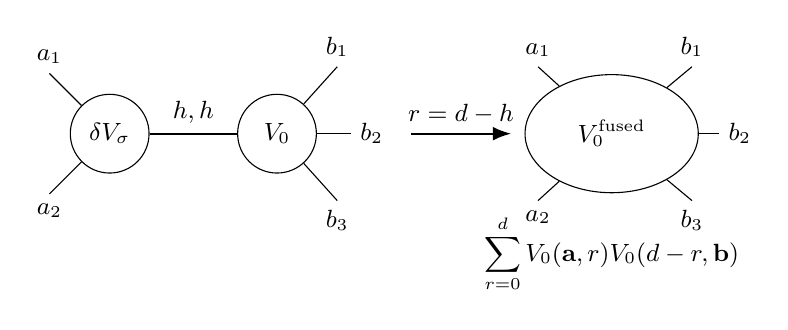
\begin{tikzpicture}[scale=.85,>=Latex,every node/.style={font=\small}]
\node[circle,draw,minimum size=10mm] (m) at (0,0) {$\delta V_\sigma$};
\node[circle,draw,minimum size=10mm] (c) at (2.5,0) {$V_0$};
\draw[thick] (m)--node[above]{$h,h$}(c);
\draw (m)--(-.9,.9) node[above]{$a_1$};
\draw (m)--(-.9,-.9) node[below]{$a_2$};
\draw (c)--(3.4,1) node[above]{$b_1$};
\draw (c)--(3.6,0) node[right]{$b_2$};
\draw (c)--(3.4,-1) node[below]{$b_3$};
\draw[->,thick] (4.5,0)--node[above]{$r=d-h$}(6,0);
\node[draw,ellipse,minimum width=22mm,minimum height=15mm] (f) at (7.5,0) {$V_0^{\mathrm{fused}}$};
\draw (f)--(6.4,1) node[above]{$a_1$};
\draw (f)--(6.4,-1) node[below]{$a_2$};
\draw (f)--(8.7,1) node[above]{$b_1$};
\draw (f)--(9.1,0) node[right]{$b_2$};
\draw (f)--(8.7,-1) node[below]{$b_3$};
\node at (7.5,-1.8) {$\displaystyle\sum_{r=0}^{d}V_0(\mathbf a,r)V_0(d-r,\mathbf b)$};
\end{tikzpicture}

\caption{A selected high incidence joins a moving trace (left disk)
to a constant trace. The original covariant labels agree, $h,h$.
Reflection changes only the left label to $r=d-h$. The complete
metric then pairs $r$ with $d-r$ and fuses the disks in their
boundary order. Every other arm remains in the same contraction.
The picture depicts the tensor calculation used for an upper bound.}
\label{ms:reflection-figure}
\end{figure}

We explain how this component statement is used in the original
tree. A circle vertex, including its fixed signed crossing and
typed turn, converts the actual incoming spectral norm into
\eqref{ms:incoming} by Lemma~\ref{ms:coupon-bound}. A maximal bare
component uses Theorem~\ref{ms:component} and preserves its full
clean low profile. Thus a small spectral-norm error is converted
to a coefficient cone at a circle interface, where the exact
extractor proves that conversion. It is never converted by an
unsupported inversion of the Newton coefficient matrix inside a
bare component. The mutual induction terminates because the
original reduced graph is a finite tree. The root budgets of
\cite[Corollary 7.5]{Newton} identify its accumulated pressure
with $F_0$, retaining every additive constant.

This also gives fresh angular localization at any exposed circle.
The clean output-probe profile is $f_A(1-u)+g(u)+\sum c_j$, with a
unique maximizing $u\in(0,1/2)$. Outside a compact interval about
it there is a strict loss. Within it the low Newton angular estimate
\cite[Lemma 7.2]{Bounds} gives a negative quadratic angular term.
Errors have a strict spectral-norm gap, so complete Hermite
conditioning and the degree-$d$ Bernstein bound absorb them on a
sufficiently small complex strip. This uses the actual accumulated
pressure and works for an entirely bare-rooted expression by
exposing any original circle through the typed adjunction. For
$H=2$ the same exact pairing is the two-leaf pure source; no
nonexistent bare component is inserted.

\section{The original finite wire packet}\label{ms:packet}
We now construct the packet in Theorem~\ref{ms:packet-main}. Let
$J_b$ be the number of bare vertices and $E=H+J_b-1$ the number
of physical edges. Denote the sums of the circle and bare valences
by $D_c,D_b$, so $D_c+D_b=2E$.

The exact positive product coefficient, from the finite Newton
calculus \cite[Theorem 3.3]{Newton}, is
\begin{equation}\label{ms:gate}
 \mu_{ij}^{r}=\frac{S_{i+j}S_r}
 {S_iS_jS_{r-i}S_{r-j}S_{i+j-r}},\qquad
 i+j\le d,\quad\max(i,j)\le r\le i+j,
\end{equation}
and is zero outside this support. At a bare vertex with ordered
labels $n_1,\ldots,n_D$, put $r_1=n_1$, $r_{D-1}=d-n_D$.
Associativity within this one polynomial algebra gives
\begin{equation}\label{ms:resolved-trace}
 \phi_0(\prod_{a=1}^D e_{n_a})
   =\sum_{r_2,\ldots,r_{D-2}}
                   \prod_{a=2}^{D-1}\mu_{r_{a-1},n_a}^{r_a}.
\end{equation}
The last pairing with $e_{n_D}$ has coefficient one. There are
$D-3$ hidden variables and $D-2$ gates, not an extra closing
variable. The physical edge labels and these hidden labels are
independent integer coordinates before inequalities are imposed.
Their number and the gate count are
\begin{equation}\label{ms:dimension}
 K=E+D_b-3J_b,\qquad G=D_b-2J_b,
 \qquad -D_c-\tfrac32G+\tfrac12K=\tfrac32(1-H).
\end{equation}
All other indices are integral affine functions of them, with
the literal complements $d-n=N(1-n/N)-1$. The lattice is
$\mathbb Z^K$ for both parities. The tree creates no additional
closing constraint or lattice-index Gaussian factor.

\subsection{The absolute action and the original window}
For $E_0=\prod_{a=1}^D e_{n_a}$ with all $n_a\le m$, the complete
ordinary-circle trace is
\begin{equation}\label{ms:circle-positive}
 \phi_0(L_NE_0)=N\sum_{r=0}^{N-1}E_0(c_r),\qquad
 N(\pi/4)^D E_0(-2)\le\phi_0(L_NE_0)\le N^2E_0(-2).
\end{equation}
The root sum is the complete trace formula of
\cite[Section 6]{Meridian}. Its terms are nonnegative. At odd
levels the node $-2$ proves the lower bound with constant one.
At even levels the nearest node satisfies
\[
 \frac{e_n(-2\cos(\pi/N))}{e_n(-2)}
 =\prod_{a=0}^{n-1}
 \frac{\cos(a\pi/N)\cos((a+1)\pi/N)}
      {\cos^2((a+1/2)\pi/N)}
 \ge\frac N2\tan\frac\pi{2N}\ge\frac\pi4.
\]
Each ratio in the product is at most one, and its endpoint value
is the displayed telescoping sine product. This proves both parity
bounds without a simple-node assumption at even levels.

The pure leaf has exact coefficients
$[e_r]h_N=N^2S_{2r}/S_r^4$ for $r\le m$, and zero otherwise:
the root sum picks the zero Laurent coefficient because $r<N$;
high $e_r$ vanish at every complete node. Expanding $E_0$ by
\eqref{ms:gate} is therefore the same positive expansion of
$\phi_0(L_NE_0)$ obtained by adjoining that leaf. Uniform
factorial rates and polynomial state counting in
\eqref{ms:circle-positive} identify its conditional maximum
exactly as $\sum_a g(n_a/N)$. At the original strict state the
eliminated variables have negative definite Hessian. Analytic
elimination consequently identifies this function and all its
derivatives near the projected state, including its additive
constant.

The grouped zero-angle action is thus
\begin{equation}\label{ms:grouped-action}
 \mathcal A(\mathbf y,0)=\sum_{\text{bare gates}}m(x,y,z)
                  +\sum_{v\text{ circle}}\sum_{e\ni v}g(x_e).
\end{equation}
Its unique maximum is the original $F_0$. Its Hessian in the
primitive coordinates is negative definite: each circle incidence
is covered by $g''<0$, and every other variable by a strict gate
whose Hessian was proved negative in \eqref{ms:gate-atoms}.
The original complete positive expansion gives a strict compact
complement gap, including its closed faces.

Choose a small rectangular box $\mathcal W$ about this maximum.
All gate factorial arguments are bulk, every circle-incident label
lies in a compact subinterval of $(0,1/2)$, and the incident sum
at each bare vertex is greater than one by a fixed amount. The
last assertion also follows by summing $x+y-z>0$ over its gates.
Lemma~\ref{ms:deletion} makes all bare physical labels strictly
low except for the internal edge of the entire two-trivalent-hub
component, which is half. Keep that edge in a compact subinterval
of $(0,1)$; both cubic traces are exactly unchanged there. Hidden
unturned indices need not be low. Every integer point of the
entire box is supported for all sufficiently large $N$.

Before continuing any angle, discard the component errors of
Theorem~\ref{ms:component}. For the clean contraction the actual
fixed-power circle trace satisfies
\begin{equation}\label{ms:fixed-power-positive}
 |\phi_\sigma(R_\sigma^n E_0)|
       \le C_{n,R,D}N\phi_0(L_NE_0).
\end{equation}
Indeed at a shifted root the angular imaginary part is $O(1/N)$.
Positive Laurent coefficients bound $|E_0|$ there by $C E_0(-2)$;
the fixed-power chirp has bounded modulus. The exact root formula
gives $C N^2E_0(-2)$ on a larger parameter circle avoiding
$\sin2\pi\sigma=0$. Divide by \eqref{ms:circle-positive} and
use the maximum principle for the whole holomorphic trace to
include collisions. Fixed nonreal compacts use the root formula
directly. Constant orientation types retain their recorded scalar.
Thus the clean resolved sum outside $\mathcal W$ has the original
positive compact gap. This bounds arbitrary subsets of the
resolved positive sum, rather than inferring an uncontracted
estimate from a scalar norm. All these source losses are fixed
before the powers and the meridian compact.

The retained exact packet is
\begin{equation}\label{ms:finite-packet}
 B_N(\boldsymbol\tau,s)=
 \sum_{\mathbf k/N\in\mathcal W}
 \left(\prod_g\mu_{N,g}\right)
 \left(\prod_{v\text{ circle}}\prod_{e\ni v}
                    e_{n_e}( -2\cos\tau_v)\right)
 \left(\prod_e\gamma_{e,N}(s)\frac{H_N(s)}{W_{n_e}(s)}\right).
\end{equation}
It is separately even and periodic in every angle. Crossing
chirps and sine trace factors are not part of this definition.

\subsection{A holomorphic interpolation of this finite sum}
Use the fixed canonical $G_N$ of \cite[Lemma 2.1]{Asymptotics},
which interpolates $S_k$, satisfies its sine shift and has uniform
bulk expansions with all fixed derivatives. For fixed $c$,
\begin{equation}\label{ms:factorial-bulk}
 G_N(Nx+c)=\sqrt{2N\sin\pi x}\,e^{NJ(x)}
              (2\sin\pi x)^c(1+O(N^{-1})).
\end{equation}
Replace every factorial in \eqref{ms:gate} by this function at
its exact affine argument. For a circle incidence set
$u=N\tau/(2\pi)$ and
\begin{equation}\label{ms:circle-interpolant}
 \mathcal E_N(x,\tau)=
 \frac{G_N(d/2+u)G_N(d/2-u)}
 {G_N(d/2-Nx+u)G_N(d/2-Nx-u)G_N(Nx)^2}.
\end{equation}
The shift identity proves equality with $e_n(-2\cos\tau)$ at
$x=n/N$. Keeping $d/2=N/2-1/2$ in
\eqref{ms:factorial-bulk} gives
\begin{align}
 \mathcal E_N(x,\tau)&=
   \frac{e^{Nb(x,\tau)}}{2N\sin\pi x}(1+O(N^{-1})),\label{ms:circle-bulk}\\
 b(x,\tau)&=\int_0^x\log(2\cos2\pi t+2\cos\tau)\,dt-2J(x).
\end{align}
The branch continues the positive real integrand at $\tau=0$;
$b(x,0)=g(x)$. An index $N\ell+c$ contributes the amplitude
$e^{c b_x(\ell,\tau)}$. All these fixed offsets are retained.

The edge interpolation is exactly \eqref{ms:exact-insertion}:
the sine shift and $G_N(s)G_N(-s)=1/H_N(s)$ give
$\mathcal I_N(n/N,s)=H_N(s)/W_n(s)$. On the fixed bulk tube,
\begin{equation}\label{ms:insertion-first}
 \mathcal I_N(x,s)=1-\frac{\pi s^2}{N}\cot\pi x+O(N^{-2}).
\end{equation}
In fact, if $L_N=\log G_N$, then
$2L_N(Nx)-L_N(Nx-s)-L_N(Nx+s)
=-s^2L_N''(Nx)+O(N^{-3})$ and
$L_N''(Nx)=\pi\cot(\pi x)/N+O(N^{-2})$.

Let $\mathcal A(\mathbf y,\boldsymbol\tau)$ be the sum of the
gate actions and these $b$'s. Dividing the exact interpolated
summand by $\Gamma_{e,N}=\prod_e\gamma_{e,N}$ gives
\begin{equation}\label{ms:summand}
 N^{-D_c-3G/2}\beta_N(\mathbf y,\boldsymbol\tau)
 e^{N\mathcal A(\mathbf y,\boldsymbol\tau)}
                   \prod_e\mathcal I_N(n_e/N,s),
\end{equation}
where $\beta_N=\beta+O(N^{-1})$ is holomorphic and
$\beta(\mathbf y^*,0)>0$. The implicit function theorem gives a
unique local wire saddle $y_*(\boldsymbol\tau)$ and invertible
$Q=-\mathcal A_{yy}(y_*,\boldsymbol\tau)$, with $Q(0)>0$.

Here is the finite-sum justification of the Gaussian. Enclose each
retained integer interval by a rectangle with half-grid vertical
sides and horizontal heights $\pm h$. The product residue formula
with kernels $\pi N\cot(\pi Nz)$ is exactly the lattice sum.
On a vertical side $|\cot|\le1$, while on the horizontal sides
\[
 \cot(\pi N(x\pm\ii h))=\mp\ii+O(e^{-2\pi Nh}).
\]
At zero angles the phase gain under the imaginary shift is at
most $C h^2$ and the real boundary has a fixed loss $\delta$.
Choose $h$ with $C h^2<\min(\delta/4,\pi h)$, then shrink the
angular polydisk. Every vertical side and every nonconstant
cotangent mode is exponentially smaller. The constant terms give
$N^K$ times the real-box integral; its endpoint displacements of
$O(1/N)$ have the same boundary loss. Translate that box to its
complex saddle. Its connecting sides retain the loss, and its real
tangent plane has negative real Hessian. Gaussian expansion gives
\[
 \Psi(\boldsymbol\tau)=\mathcal A(y_*,\boldsymbol\tau),\qquad
 a(\boldsymbol\tau)=
 \frac{(2\pi)^{K/2}\beta(y_*,\boldsymbol\tau)}{\sqrt{\det Q}}.
\]
The square root starts at the positive real Gaussian and never
vanishes on a smaller polydisk. Equation~\eqref{ms:dimension}
gives the claimed power of $N$. Odd Gaussian terms integrate to
zero, so the relative remainder is $O(1/N)$, uniformly holomorphic.
Separate evenness and uniqueness imply
$\mathcal A_{y\tau_v}(\mathbf y,0)=0$. Direct differentiation
gives $b_{\tau\tau}(x,0)=-\tan(\pi x)/(2\pi)$, proving the
diagonal angular Hessian in Theorem~\ref{ms:packet-main}.

\subsection{The whole real angular cube}
For $n/N$ in a fixed compact subset of $(0,1/2)$, the exact product
gives the following strengthening of \cite[Lemma 7.2]{Bounds}:
\[
 |e_n(-2\cos(t+\ii y))|
 \le N^A e^{Ng(n/N)-Nct^2+NCy^2},\qquad |t|\le\pi.
\]
Indeed near zero the logarithm of
$e_n(-2\cos w)/e_n(-2)$ is even, has second derivative
$-2\sum_{j<n}(c_j+2)^{-1}\le-cN$, and all fixed higher
derivatives are $O(N)$ on one uniform zero-free disk. Taylor's
formula gives $-cNt^2+CNy^2$ there. On the remaining compact
real interval the imported lemma gives a strict real gap, including
sampled numerator zeros, by truncated logarithmic Riemann upper
sums. Shrink the complex height and reduce $c$ so a fixed part of
that gap remains; it absorbs the uniform $e_N=o(1)$ error in
the imported estimate. Finally
$e_n(-2)=\exp(Ng(n/N)+O(\log N))$ supplies the polynomial
prefactor. Thus no polynomial error bound at arbitrary numerator
collisions is assumed. All bare factors in
\eqref{ms:finite-packet} are nonnegative and the edge ratios are
bounded. The positive zero-angle sum has rate $F_0$ and polynomial
prefactor by the Gaussian just proved. Every circle has an incident
edge, so summing the bound proves \eqref{ms:packet-strip} with a
positive loss in every angle. Endpoints translated by $O(1/N)$
retain it by periodicity: the squared distance to $2\pi\mathbb Z$
changes by $O(1/N)$. Fixed derivatives cost powers of $N$ by Cauchy
estimates on radius-$1/N$ circles. This completes the proof of
Theorem~\ref{ms:packet-main}, including its actual finite source
error before any crossing contour is moved.

\section{All charges of the original crossing traces}\label{ms:filling}
The powers $n_v$ are fixed signed integers. In the primitive filling
convention they are $n_v=\epsilon_v-2p_v$; odd powers are included.
This section proves Theorem~\ref{ms:filled-main} analytically. It
does not identify a geometric action.

\subsection{The full finite functional and its currents}
For an even polynomial $f(\tau)=f^\sharp(-2\cos\tau)$ define
$\mathcal D_{n,\sigma,N}f=\phi_\sigma(R_\sigma^n f^\sharp)$.
The full crossing data in \cite[Proposition 6.1 and equation (6.4)]{Meridian}
give, with $\eta=(-1)^d$,
\begin{align}
 \mathcal D_{n,\sigma,N}f
 &=\frac{\eta N C_{N,n}(\sigma)}{\sin2\pi\sigma}
 \sum_{r=0}^{N-1}\sin\tau_r\,f(\tau_r)
                  e^{\ii nN\tau_r^2/(4\pi)},\label{ms:trace}\\
 \tau_r&=\frac{2\pi}{N}(d/2+\sigma-r),\qquad
 C_{N,n}(\sigma)=q^{n(d^2/4-\sigma^2/2)}.
\end{align}
This is first written off the collisions. Its removable limit is
the full Hermite functional, not just the node values. In
particular inverse powers use the same formula.

Introduce independent formal grid parameters $\sigma_v$ temporarily;
the actual assignments are $0,s,-s$. If $\zeta_N$ is the original
closing and framing scalar and $\rho_{v,N}$ the reference scalar
for its orientation type, set $\widehat\zeta_N=\zeta_N\prod_v\rho_{v,N}$.
The exact source reduction already proved has the form
\begin{equation}\label{ms:source-to-functional}
 F_N(q^s)=\widehat\zeta_N(s)H_N(s)
       \left(\prod_v\mathcal D_{n_v,\sigma_v,N}^{(v)}\right)
       B_N(\boldsymbol\tau,s)
       +O(N^A e^{N(F_0-\eta_0)}).
\end{equation}
Each factor acts in its own variable; this is tensor evaluation,
not commutation of physical crossing operators. Edge scalars are
already in $B_N$ and are not counted in $\widehat\zeta_N$.

Choose $R<R'<1$, $R'\ne1/2$, and initially take
$|\sigma_v|=R'$. For one coordinate use the exact pole kernel
\[
 K_\sigma(\tau)=\frac{\ii N e^{\ii N\tau}}
              {e^{\ii N\tau}-\eta e^{2\pi\ii\sigma}}.
\]
It has residue one at precisely the shifted grid points. Integrate
it times $\sin\tau f(\tau)e^{\ii nN\tau^2/(4\pi)}$ around a
rectangle translated by $2\pi\sigma/N$ enclosing those $N$ poles.
On its vertical sides
\[
 K_\sigma(\pm\pi+\ii v+2\pi\sigma/N)
                  =\frac{\ii N e^{-Nv}}{1+e^{-Nv}}.
\]
On horizontal sides expand the denominator geometrically. After
reflecting the upper side by $\tau\mapsto-\tau$, the odd sine
factor pairs the positive and negative frequencies. Their parameter
multiplier is
\[
 \frac{e^{2\pi\ii\ell\sigma}-e^{-2\pi\ii\ell\sigma}}
      {e^{2\pi\ii\sigma}-e^{-2\pi\ii\sigma}}
       =U_{\ell-1}(\cos2\pi\sigma).
\]
The grid sign and the contour orientations give
\begin{equation}\label{ms:charges}
 c_{\ell,N}(\sigma)=\eta^{\ell-1}
                 U_{\ell-1}(\cos2\pi\sigma),\qquad c_{1,N}=1.
\end{equation}
The zero-frequency real integral vanishes by oddness. Its endpoint
currents, and the connectors from the translated endpoints, remain
in the contour identity. This calculation explains why replacing
the repeated-node functional by values would lose the factor
$c_{\ell,N}(0)=\eta^{\ell-1}\ell$.

Choose $t_0>0$ small and put
$L_v=\lfloor t_0|n_v|\rfloor$, $y_v=A_0t_0/|n_v|$.
The finite real functional retained from this exact contour is
\begin{equation}\label{ms:finite-charges}
 \mathcal P_{n,\sigma,N}^{L}f
 =-\frac{N^2 C_{N,n}(\sigma)}{\pi\ii}
 \sum_{\ell=1}^{L}c_{\ell,N}(\sigma)
 \int_{-\pi}^{\pi}\sin\tau f(\tau)
             e^{\ii nN\tau^2/(4\pi)-\ii\ell N\tau}\,d\tau.
\end{equation}
Here is a uniform bound for what was omitted. On the lower
horizontal side the packet and chirp have real rate at most
\[
 F_0-ct^2+\frac{|n||t|y}{2\pi}-\ell y+Cy^2.
\]
The maximum of the two $t$ terms is $n^2y^2/(16\pi^2c)$.
For $\ell>L$ the resulting upper rate is
\[
 F_0+t_0^2\left(\frac{A_0^2}{16\pi^2c}-A_0
                         +\frac{CA_0^2}{n^2}\right)
                         -(\ell-L-1)y.
\]
First choose $A_0$ so its first positive term is at most $A_0/4$,
then a lower threshold for $|n|$ so the last one is also at most
$A_0/4$. The loss is at least $A_0t_0^2/2$, independently of $n$.
The bound $|c_{\ell,N}(\sigma)|\le\ell e^{2\pi R'(\ell-1)}$
makes the remaining geometric sum convergent for all sufficiently
large $N$. Constants depending on fixed $n$ do not change this rate.

At the vertical endpoints the angular loss is fixed. Their chirp
cost is $O(N|n|y)=O(Nt_0)$, and the retained-charge connector cost
is $O(NLy)=O(Nt_0^2)$. Decrease $t_0$ to preserve the loss. This
also controls the zero-mode current. All spectator variables can
remain real or on their physical translated grids: those grid
heights are $O(1/N)$ and their fixed chirps have bounded modulus.
Use the exact telescoping identity
\[
 \prod_v\mathcal D_v-\prod_v\mathcal P_v
 =\sum_j(\prod_{v<j}\mathcal P_v)
                   (\mathcal D_j-\mathcal P_j)
                   (\prod_{v>j}\mathcal D_v).
\]
The other $\mathcal P$'s are finite real integrals of polynomial
operator cost, and the other $\mathcal D$'s are finite physical
grid sums. Thus every telescoping term has rate $F_0-\gamma$ for
one fixed $\gamma>0$. No spectator is moved to a slope-dependent
complex height during another coordinate's tail estimate.

The whole trace-minus-finite-approximation is holomorphic in each
$\sigma_v$. Apply the maximum principle successively to extend
the estimate from the parameter circles to $|\sigma_v|\le R$.
This includes all normal limits at $0,\pm1/2$. For any fixed
upper-half-plane compact use the same translated contour directly;
its sine denominator is bounded away from zero and its endpoint
translation is still $O(1/N)$. Constant vertices can independently
be brought to zero by the preceding disk argument. Fixed
derivatives follow on smaller compacts.

\subsection{A common critical branch for every retained charge}
After truncating the real integral to a small angular box, with
fixed loss, its phase is
\[
 T_{\boldsymbol\ell}(\boldsymbol\tau)
 =\Psi(\boldsymbol\tau)
       +\frac{\ii}{4\pi}\sum_v n_v\tau_v^2
       -\ii\sum_v\ell_v\tau_v.
\]
Set $\varepsilon_v=1/n_v$, $t_v=\ell_v/n_v$. Its critical equation
and a removable stationary expression are
\begin{align}
 \tau_v&=2\pi t_v+2\pi\ii\varepsilon_v\Psi_v(\boldsymbol\tau),
       \label{ms:joint-critical}\\
 W(\mathbf t,\boldsymbol\varepsilon)
 &=\Psi(\boldsymbol\tau)
                -\ii\pi\sum_v\varepsilon_v\Psi_v(\boldsymbol\tau)^2.
\end{align}
The implicit function theorem gives one holomorphic branch on a
fixed polydisk about $(0,0)$. The critical action is
$-\ii\pi\sum t_v^2/\varepsilon_v+W$; the first term is purely
imaginary for the real signed data. Separate evenness makes $W$
even in each $t_v$. At $\boldsymbol\varepsilon=0$,
$W(\mathbf t,0)=\Psi(2\pi\mathbf t)$, so
$\partial_{t_v^2}\Re W(0,0)=-2\pi^2 a_v$.
Shrink the polydisk until all these derivatives are at most
$-\pi^2a_v$. Integration in the squared coordinates gives
\begin{equation}\label{ms:joint-loss}
 \Re T_{\boldsymbol\ell}(\boldsymbol\tau_{\boldsymbol\ell})
 \le\Re T_{\mathbf1}(\boldsymbol\tau_{\mathbf1})
       -\sum_v\frac{\pi^2a_v}{n_v^2}(\ell_v^2-1).
\end{equation}
Choose $t_0$ inside this polydisk and then increase the single
lower threshold for all $|n_v|$. This covers every retained charge
without a restriction on their slope ratios.

Write $\Psi_v=\tau_v Q_v(\tau_1^2,\ldots,\tau_H^2)$, with
$\Re Q_v<0$ in that neighborhood. Then
\begin{equation}\label{ms:critical-angle}
 \tau_{\boldsymbol\ell,v}=
 \frac{2\pi t_v}{1-2\pi\ii\varepsilon_v Q_v},\qquad
 \Im\tau_{\boldsymbol\ell,v}
 =\frac{4\pi^2\ell_v\Re Q_v}
              {n_v^2|1-2\pi\ii\varepsilon_vQ_v|^2}<0.
\end{equation}
Every angle and every sine in the amplitude is nonzero. Translate
the small real box to this critical point. The real part of its
Hessian on real tangent vectors is that of $\Psi''$, since the
chirp Hessian is purely imaginary, and stays negative definite.
The connectors preserve the face loss: their heights are at most
$C|t_v|/|n_v|$, their chirp cost on a face of size $\rho$ is at
most $CN\rho|t_v|$, and their Fourier factors decrease under the
downward displacement. Choose $t_0$ small compared with the fixed
face loss before increasing the slope threshold.

Use the holomorphic packet expansion on this contour, not a real
pointwise remainder. Gaussian integration and
\eqref{ms:dimension} give for the entire retained contraction
\begin{equation}\label{ms:filled-packet}
 \left(\prod_v\mathcal D_v\right)B_N
 =\left(\prod_v C_{N,n_v}(\sigma_v)\right)
   \Gamma_{e,N}(s)N^{3/2}D_{\mathbf n}
   e^{N T_{\mathbf1}(\boldsymbol\tau_{\mathbf1})}
                         (1+O(N^{-1})),
\end{equation}
where
\[
 D_{\mathbf n}=\left(-\frac1{\pi\ii}\right)^H(2\pi)^{H/2}
 \frac{a(\boldsymbol\tau_{\mathbf1})\prod_v\sin\tau_{\mathbf1,v}}
 {\sqrt{\det[-T_{\mathbf1}''(\boldsymbol\tau_{\mathbf1})]}}\ne0.
\]
The branch is fixed by the translated real Gaussian. There are
only finitely many charges for fixed powers. Equation
\eqref{ms:joint-loss} suppresses every one except $\mathbf1$,
whose coefficient is exactly one by \eqref{ms:charges}. The
reflected signs have already been paired, leaving no equal-action
terms with an unexamined relative sign. The wire Hessian and this
angular Schur complement are invertible, hence so is the full
joint Hessian.

The first action tends to $F_0$ as $\max_v|1/n_v|\to0$.
Increase the common threshold to put its real part above $F_0$
minus half each fixed source, contour-tail and off-window loss.
Those additive errors are then negligible. The charge-dependent
losses were instead compared to this same filled action in
\eqref{ms:joint-loss}; a smallest local loss is never compared
with a total complete-to-filled drop.

Finally restrict $\sigma_v$ to the actual types. The finite scalar
ledger \cite[Proposition 8.1]{Meridian}, which retains every typed
turn, monodromy, crossing carrier and framing correction, says
\[
 \frac{\widehat\zeta_N(s)}{\widehat\zeta_N(0)}
 \Gamma_{e,N}(s)\prod_v q^{-n_v\sigma_v(s)^2/2}
                       =q^{a(D)s^2/2},\qquad
 a(D)=-w(D)-\sum_v n_v.
\]
There is still exactly one main-cut factor $H_N$ in
\eqref{ms:source-to-functional}. This proves
\eqref{ms:filled-leading}. Removing these exact scalars leaves
only the product of \eqref{ms:exact-insertion} on the original
physical edges in the joint integral. The zero-meridian amplitude
and all its offsets are common, so no first-order scalar is hidden
in that assertion. Every choice of an exponential margin or a
slope threshold preceded the choice of a meridian compact; only
bounded factors and starting levels depend on that compact.


\begin{thebibliography}{9}
\bibitem{Meridian}\emph{Exact Newton calculus for tangles with a moving meridian}, companion paper,
\href{https://sashakolpakov.github.io/murakamis_dream/papers/meridian-tangles.pdf}{repository edition}.
\bibitem{Newton}\emph{Newton coefficients and positive sources for Conway tangles}, companion paper,
\href{https://sashakolpakov.github.io/murakamis_dream/papers/newton-tangles.pdf}{repository edition}.
\bibitem{Profiles}\emph{Stationary profiles of strict Newton trees}, companion paper,
\href{https://sashakolpakov.github.io/murakamis_dream/papers/strict-newton-profiles.pdf}{repository edition}.
\bibitem{Bounds}\emph{Spectral estimates for Conway tangle sources}, companion paper,
\href{https://sashakolpakov.github.io/murakamis_dream/papers/conway-source-bounds.pdf}{repository edition}.
\bibitem{Asymptotics}\emph{Holomorphic source asymptotics and volume limits for strict Conway compositions}, companion paper,
\href{https://sashakolpakov.github.io/murakamis_dream/papers/conway-asymptotics.pdf}{repository edition}.
\end{thebibliography}
\end{document}
